
%%%%%%%%%%%%%%%%%%%%%%% file typeinst.tex %%%%%%%%%%%%%%%%%%%%%%%%%
%
% This is the LaTeX source for the instructions to authors using
% the LaTeX document class 'llncs.cls' for contributions to
% the Lecture Notes in Computer Sciences series.
% http://www.springer.com/lncs       Springer Heidelberg 2006/05/04
%
% It may be used as a template for your own input - copy it
% to a new file with a new name and use it as the basis
% for your article.
%
% NB: the document class 'llncs' has its own and detailed documentation, see
% ftp://ftp.springer.de/data/pubftp/pub/tex/latex/llncs/latex2e/llncsdoc.pdf
%
%%%%%%%%%%%%%%%%%%%%%%%%%%%%%%%%%%%%%%%%%%%%%%%%%%%%%%%%%%%%%%%%%%%


\documentclass[runningheads,a4paper]{llncs}


\setcounter{tocdepth}{3}
\usepackage{graphicx}
%
\usepackage{mathptmx}      % use Times fonts if available on your TeX system
%
% insert here the call for the packages your document requires
\usepackage{latexsym}
\usepackage{url}
\usepackage{changepage}
\usepackage{amssymb,amsmath}
\usepackage[colorlinks,citecolor=blue,linkcolor=blue]{hyperref}
\usepackage{color}
\usepackage{mdwlist}
\usepackage{algorithm}
\usepackage{algorithmic}
\renewcommand{\algorithmicrequire}{ \textbf{Input:}} %Use Input in the format of Algorithm
\renewcommand{\algorithmicensure}{ \textbf{Output:}} %UseOutput in the format of Algorithm
%\spnewtheorem{definition}{Definition}{\bf}{\rm}
\spnewtheorem{hypothesis}{Hypothesis}{\bf}{\rm}

\usepackage{url}
\urldef{\mailsa}\path|{xsongx,jtaotang,tingwang}@nudt.edu.cn| 
%\urldef{\mailsb}\path|jtaotang,|
%\urldef{\mailsc}\path|tingwang}@nudt.edu.cn|    
\newcommand{\keywords}[1]{\par\addvspace\baselineskip
\noindent\keywordname\enspace\ignorespaces#1}

\begin{document}

\mainmatter  % start of an individual contribution

% first the title is needed
\title{Integrating Topic Related Opinions of Users on Social Media: a Separate Way}

% a short form should be given in case it is too long for the running head
%\titlerunning{Lecture Notes in Computer Science: Authors' Instructions}

% the name(s) of the author(s) follow(s) next
%
% NB: Chinese authors should write their first names(s) in front of
% their surnames. This ensures that the names appear correctly in
% the running heads and the author index.
%
\author{Xie Songxian%
%\thanks{Please note that the LNCS Editorial assumes that all authors have used
%the western naming convention, with given names preceding surnames. This determines
%the structure of the names in the running heads and the author index.}%
\and Tang Jintao\and Wang Ting}
%
%\authorrunning{Lecture Notes in Computer Science: Authors' Instructions}
% (feature abused for this document to repeat the title also on left hand pages)

% the affiliations are given next; don't give your e-mail address
% unless you accept that it will be published
\institute{School of Computer Science, National University of Defense Technology,\\
Yanwachi Street of Changsha, Hunan, China, 410073\\
\mailsa\\}
%\mailsb\\
%\mailsc\\
%\url{http://www.nudt.edu.cn}}

%
% NB: a more complex sample for affiliations and the mapping to the
% corresponding authors can be found in the file "llncs.dem"
% (search for the string "\mainmatter" where a contribution starts).
% "llncs.dem" accompanies the document class "llncs.cls".
%

\toctitle{Lecture Notes in Computer Science}
\tocauthor{Authors' Instructions}
\maketitle


\begin{abstract}
Social media such as Twitter, has enabled more and more people to express their opinions on the web freely, making it an extremely valuable source for mining opinions of users about all kinds of topics. In this paper we study how to automatically integrate topic related opinions expressed by a user in not so well-written User-Generated Content (UGC). We propose a subjectivity model by combining topics a user talks about and his opinions towards these topics. There have been several generative topic-sentiment mixture models designed to capture sentiments and topics in text simultaneously. In constrast to generatvie models, we construct our model with LDA topic model and sentiment analysis techniques in a separate way. We compare our model and generative models in a series of experiments on Twitter data. Results show that the proposed model is effective and can generate useful aligned integrated opinion summaries of users. Futhermore, the proposed model is more suitable for social media context, thus can catch more fine-grain opinions than generative models and get better performance in a link prediction task. 
\keywords{generative model, social media, opinion mining, subjectivity model}
\end{abstract}

\section{Introduction}
\label{sec1}

With the rise of text-based social media such as Twitter, millions of users are more and more willing to publish online short messages to express their opinions on a great variety of topics they are interested in. The wide coverage of topics, dynamics of discussion, and abundance of opinions imbeded in the social media data make them extremely valuable for mining users' opinions about all kinds of topics (e.g., products, political figures, etc.), which in turn can enable a wide range of applications, such as opinion search for ordinary users, opinion tracking for business intelligence, and user behavior prediction for targeted advertising. 
However, with such a large scale of information source, it is quite challenging to integrate and digest all the opinions from different users. For example, a query ``iPhone'' on Twitter (as of Jan. 14, 2014) returns 830,879 tweets of 231,233 users, suggesting that there are many users have expressed opinions more than once about iPhone in their tweets. To enable an application to benefit from all kinds of opinions of different users, it is thus necessary to automatically integrate and present an integrated opinion summary for each user \cite{lu2008opinion}. In fact, users often publish many messages on the topics they are interested in, therefore how to find these topics and integrate opinions towards each topic poses special challenge for opinion mining related researchers.

In this paper, we propose a two-parts model ( name as subjectivity model) by incorporating topic model and sentiment analysis into one framework, in which part 1 represents topics of interest distribution of users, while part 2 represents the distribution of opinions towards these topics. Specifically, we propose a general method to solve this integration problem in three steps illustrated as in Figure~\ref{fig1}: (1) extract topics of interest from tweets of a user using user-level LDA; (2) extract separated sentiment and topic for each tweet with sentiment and topic analysis  (3) summarize and integrate the extracted opinions towards topics to form a subjectivity model for each user.
\begin{figure}[htb]
\centering
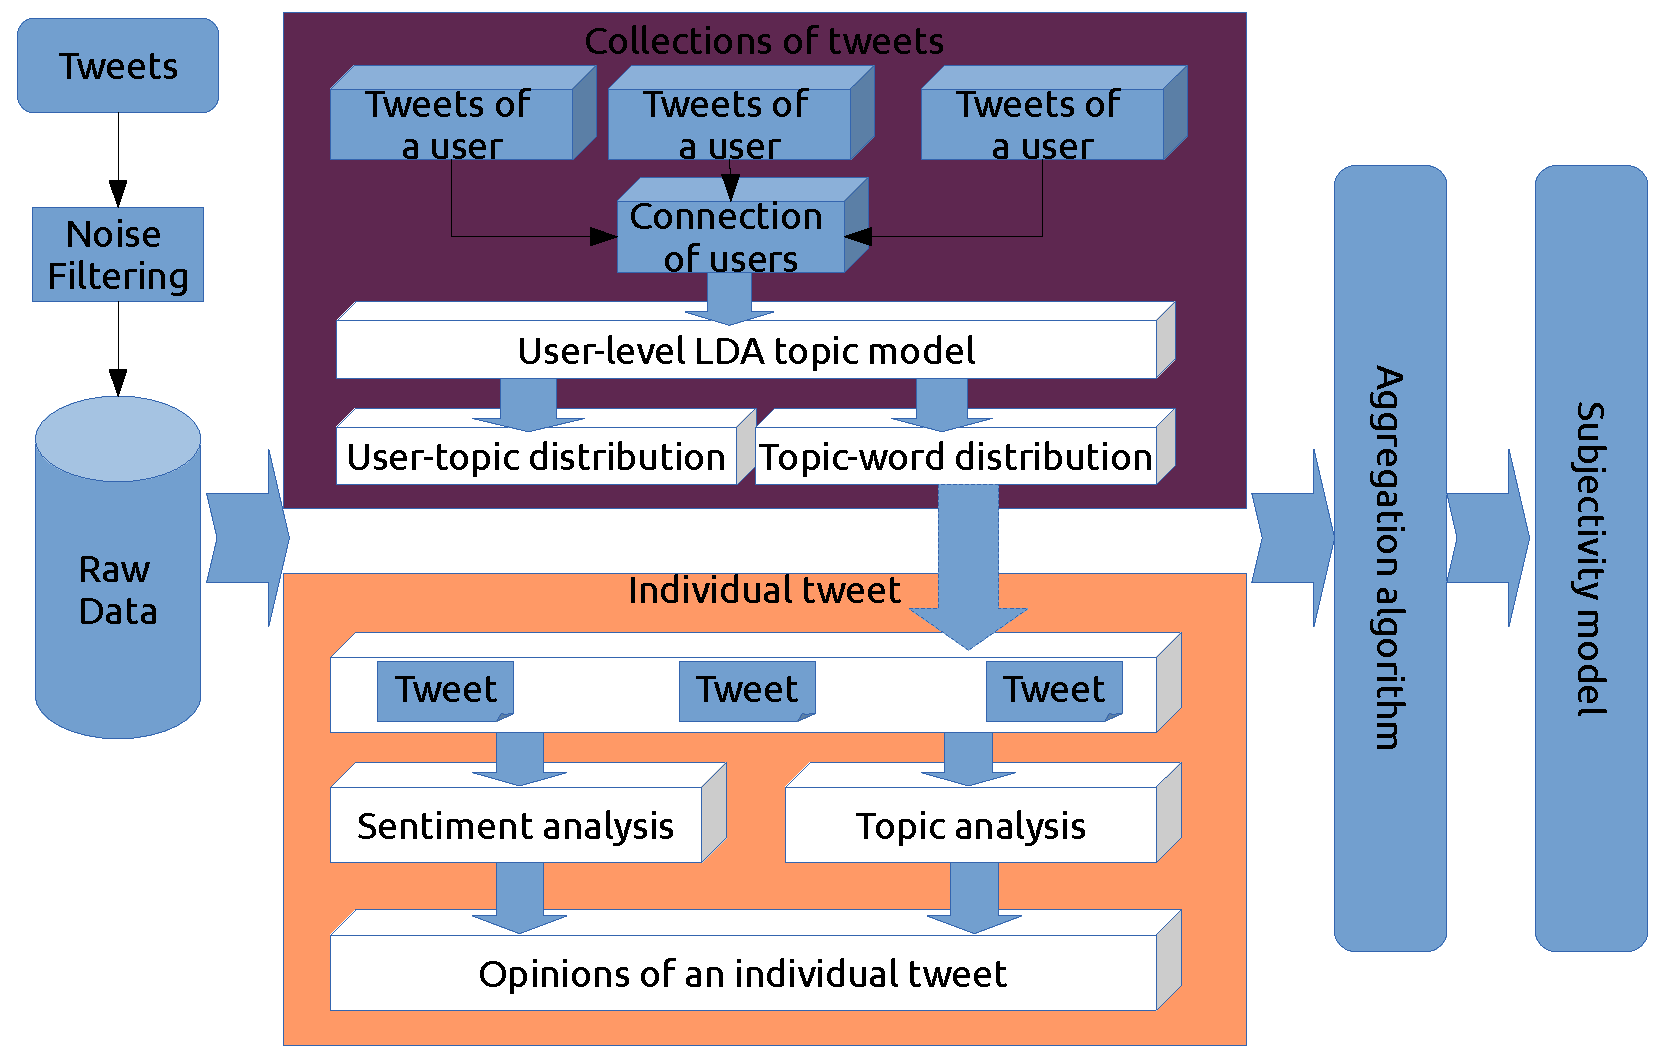
\includegraphics[width=4.2in,height=2.5in]{procedure.pdf}
\caption{Framework of two-parts subjectivity model.}
\label{fig1}
\end{figure}

Several studies have tried to combine sentiment into a unified generative topic model to mine topic related sentiments in reviews or blogsphere. Mei \emph{et al.}~\cite{mei2007topic} proposed Topic-Sentiment Mixture (TSM) model that can reveal latent topics of a blog and the topics associated sentiments. Lin \emph{et al.}~\cite{lin2009joint} proposed a Joint Sentiment/Topic (JST) model based on LDA that can detect topic and sentiment simultaneously in reviews. This paper presents a comparative study of these closely related generative models for unsupervised user level opinion mining.

This paper makes the following contributions:
\begin{itemize}
\item We define a new problem of opinion integration at user-level. To the best of our knowledge, there are few works that meet such a problem.
\item We propose a two-parts model and a separated approach for integrating opinions scattered around in tweets of a user for the topics he is interested in.
\item We evaluate the proposed method both qualitatively and quantitatively comparing with state-of-the-art generaitve models. The results show that our method is effective for integrating opinions for users and a friend recommendation task.
\end{itemize}

Collecting and digesting opinions about a topic from different users are critical for many tasks such as shopping, medical decision making, and social interactions. Our proposed method is quite general and can be applied to integrate opinions about any topic in any domain, thus potentially has many interesting applications. The rest of the paper is organized as follows. In Section 2, related works are presented, then we formally define the novel problem of opinion integration in Section 3. After that, we present our model and analyze the difference with generative model in Section 4. We discuss our experiments and results in Section 5. Finally, we conclude in Section 6.

\section{Related Works}
\label{sec2}

Sentiment analysis is a popular research area and previous researches have mainly focused on reviews or news comments \cite{pang2008opinion,liu2012sentiment}. 
Recently, there have been some works on sentiment analysis on Twitter, mainly focusing on the tweet level \cite{barbosa2010robust,davidov2010enhanced,jiang2011target,li2010micro,tan2011user}, of which, the techniques employed are generally standard tweet-level algorithms that ignore links between users. There have been also some previous works on automatically determing user-level opinions or ideology \cite{agrawal2003mining,mostafa2013more,malouf2008taking,yu2008classifying}, generally looking at information embeded in the contents that the users generate. Most of related researches mainly focused on identification of sentimental object \cite{liu2010comment}, or detection of object’s sentimental polarity \cite{zhai2011constrained} without considering the topic aspects. 

Since the introduction of LDA model \cite{blei2003latent}, various extended LDA models have been used for topic extraction from large- scale corpora at user level. Rosen-Zvi \emph{et al.}~\cite{rosen2004author} introduced the Author-Topic (AT) model, which includes authorship as a latent variable. Ramage \emph{et al.}~\cite{ramage2009labeled} introduced Labeled LDA to supervise the generation of topics via user tags. Topic models can also be utilized in sentiment analysis to correlate sentiment with topics \cite{mei2007topic,lin2009joint}. Mei \emph{et al.}~\cite{mei2007topic} and Lin \emph{et al.}~\cite{lin2009joint} incorporated topic models and sentiment analysis for reviews and blogs. However, our work attempts to integrate opinions of a user by combining topic models and sentiment analysis together into a two-parts framework.

\section{Opinion Integration Problem}
\label{sec3}

As we describe in Section~\ref{sec1}, a user usually publishes multiple messages on multiple topics when he using social media. Therefore what's the opinion of a user on a special topic can not be determined from just one tweet, but should be interated from the topic related tweets he has published. In this paper, we put forwad a new problem which is defined as \emph{Opinion Integration Problem} (OIP). We focus on user-level rather than tweet-level opinion because the end goal of opinion mining technologies is to find out what a person thinks but not what only a piece of message states, determining the opinion expressed in individual text is usually a middle step for that ultimate objective. Additionally, it is plausible that there are cases where opinions in some of a user’s tweets are genuinely ambiguous because they are restricted to be very short, but his overall opinion can be determined by looking at his collection of tweets \cite{tan2011user}. 
We show a typical scenario of user-level topic related opinion integration problem on Twitter in Figure~\ref{fig2}.
\begin{figure}[htb]
%\setlength{\belowcaptionskip}{-0.2cm} 
\centering
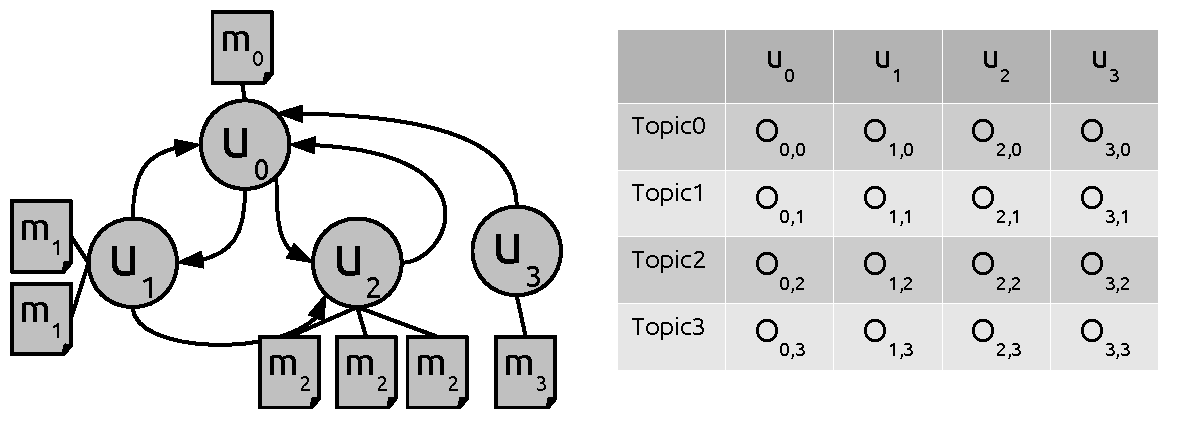
\includegraphics[width=3.8in,height=1.2in]{ego.pdf}
%\vspace{-4em}
\caption{Illustration of Opinion Integration Problem.}
\label{fig2}
\end{figure}
As denoted in the figure, a subnetwork of Twitter (users $ \left\{ u_{i} \right\} $ and their directional relations), and their associated tweets (denoted as $ \left\{ m_{i} \right\} $) are used to extract topics (denoted as $ \left\{ Topic_{j} \right\} $) and opinions (denoted as $ O_{i,j} $). Opinion $ O_{i,j} $ is not the opinion imbeded in single tweet $ m_{i} $, but the integrated opinion form from all tweets $ \left\{ m_{i} \right\} $. 

There’re two important factors that should be taken into considerations for the OIP problem. Firstly, topics of all users and tweets talks about and should be dertermined in a same topic space so as the target of opinion is normalized. Secondly but most importantly, opinions and topics are closely related, tweets of a user around some topic often cover a mixture of features related to that topic with different preferentials. Different opinions may be expressed by the user towards different features, where users may like some aspects of an topic but dislike other aspects. Therefore, how to integrate all opinions of tweets related to a topic into one opinion and represent it reasonably poses special challenge. There are different ways to meet such a challenge, generatively as TSM model or separatedly as we describe in this paper, and we will define our model and compare them in this paper. 

\section{Subjectivity Model}
\label{sec4}

In this section, we give a formal definition of the model we work with to meet the challenges of OIP problem. Usually user-level opinion is to classify each user’s sentiment on a specific topic into one of two polarities: ``Positive'' and ``Negative''. ``Positive'' means that the user supports or likes the target topic, whereas ``Negative'' stands for the opposite. However we adopt a broad ``opinion'' definition as sentiment coverage towards a topic over a fine-grain strength values to differentiate opinions of users. The notion of ``opinion'' is quite vague; we adopt this broad definition to ensure generality of the model. We frame the problem in the context of Twitter to keep things concrete, although adaptation of our model to other social-network settings is straightforward. We name our model as ``\textbf{Subjectivity Model}'' as it models the subjective information in the content generated by a user. Therefore, we give a formal definition of the subjectivity model under the context of Twitter as follows.

\subsection{Definition}
\label{definition}

Let $G=\left( V,E \right) $ denote a social network on Twitter, where $ V $ is a set of users, and $ E\subset V\times V $ is a set of follow relationships between users. For each user $ u \in V $, there is a tweets collection $ M_{u} $ denoting his message history. We assume that there is a topic space $ T $ containing all topics users in $ V $ talk about, and a sentiment valence space $ S $ to evaluate their opinions towards these topics. 
For the ``subjectivity'' of a user $ u  \in V $, we refer to both topics and opinions articulated in his tweets collection $ M_{u} $.  
\begin{definition}[Subjectivity Model]
The subjectivity model $ P \left( u \right) $ of user $ u $, is the combination of topics $\left\lbrace  t \right\rbrace $ the user talks about in topic space $T$ and his opinions $\left\lbrace O_{t}\right\rbrace $ towards each topic distributed over sentiment valence space $ S $. 
\begin{equation}
\label{usermodel}
P \left( u \right) = \lbrace \left( t, w_{u} \left( t \right), \lbrace d_{u,t} \left( s \right)|s \in S \rbrace \right) |  t \in T \rbrace
\end{equation}
where:
\begin{itemize}
\item with respect to user $ u $, for each topic $t \in T$, its weight $ w_{u} \left( t \right)$ represents the distribution of the user's interests on it, subject to $ \sum_{t=1}^{|T|}w_{u} \left( t \right)=1 $.
\item opinion of the user towards topic $t$ is modelled as a topic-dependent sentiment distribution over sentiment valence space $ S $, $O_{t}=\lbrace d_{u,t} \left( s \right)|s \in S \rbrace $, subject to $ \sum_{s=1}^{|S|} d_{u,t} \left( s \right)=1$.
\end{itemize}
\end{definition}

Subjectivity Model captures user’s subjectivity by considering both topic and opinion simultaneously. Topic weights of users are modelled by a topic distribution and users have opinion distribution on each topic over all sentiment valence space. Subjectivity Model aims at obtaining the sentiment-refined topics for investigating user-level opinion mining. Unlike previous works to do document-level sentiment analysis which either caculate the overall document sentiment or model aspect related opinions as sentiment polarity classification \cite{tan2011user}.
We now address the problems of estimating the free parameters in Subjectivity Model and inferring topic related opinions once the parameter values have been learned.

\subsection{Establishment of Subjectivity Model }
\label{establish}

According to the definition of subjectivity model , there are two distributions to model the subjectivity: the topic distribution and the opinion distribution for each topic. Both of them need to be inferred from historic content produced by users.
However, content analysis on Twitter is challenging: the volume of tweets is so huge while a single tweet is very short with limit of 140 characters, and informal languages are widely used, which make many supervised learning approaches and natural language processing techniques invalid. 
Hence effectively modeling content on Twitter requires techniques that can readily adapt to these challenges and require little supervision. 
With state-of-the-art topic model and sentiment analysis techniques, we establish subjectivity model by identifying topics and opinions in an unsupervised way simultaneously. The main advantage of our establishing framework is that it employs social-network structure to help us overcome both the paucity of textual information in short tweets and the lack of a large amount of labeled data \cite{lin2010comparative}.


\subsubsection{Topic Analysis}
\label{topic}

The topics of a tweet are latent and have to be inferred from its content.
Previous studies have tried to identify topics from tweets by finding key words \cite{chen2010short}, extracting  entities \cite{abel2011analyzing} or linking tweets to external knowledge categories \cite{macskassy2011people}, however, the sparsity is a main problem for these methods because even users have common local topics they still might refer to a topic with different vocabulary.
Works show that topic models such as \textbf{Latent Dirichlet Allocation (LDA)} model \cite{blei2003latent} have been efficient ways to characterize latent topics of large volume corpus.  
Topics of LDA are broader in concept, since a single topic consists of the whole collection of related words. 
Therefore we adopt a user-level LDA model to find latent topics for users.
To distill the topics, documents of LDA should naturally correspond to tweets content. 
As our goal is to understand the topics that each user is interested in rather than the topics each single tweet talks about, we aggregate the tweets published by each user into a single document, and replace documents of LDA with aggregated tweet documents. 
So a document stands for a user in our model, and a user can be represented as a multinomial distribution over topics, which corresponds to the topic distribution of the user's subjectivity model.

Formally, given a set of users $ U $ and the number of topics $ K $, a user $u$ ($ u \in U $) could be represented by a multinomial distribution $ \theta_{u} $ over topics with a Dirichlet prior parameterized by $ \alpha $. 
A topic $ k $ ($ k \in K $) is represented by a multinomial distribution $ \beta_{k} $ with another Dirichlet prior parameterized by $ \eta $. 
The parameters $ \theta_{u} $ and each $ \beta_{k} $ can be estimated by Gibbs sampling or variational inference.
We use variational inference-based topic model package Gensim \cite{rehurek_lrec}.

\subsubsection{Opinion Analysis}
\label{sentiment}

Users often express opinions towards their topics of interest by publishing topic-related tweets. 
In order to explore the opinions of users, we need to understand sentiment embedded in each tweet.
Sentiment analysis mainly depends on machine learning or rule-based approaches. 
Machine learning approaches often need labelled data for the training process, which is often impossible for Twitter because of the large volume of tweets and its dynamic language characteristics. Therefore we adopt rule-based approaches, which could adapt to Twitter with good flexibility by changing its particular characteristics into rules \cite{thelwall2010sentiment}.

The SentiStrength package has been built especially to cope with sentiment analysis in short informal text of social media \cite{thelwall2010sentiment}. 
It combines lexicon-based approaches with sophisticated linguistic rules adapted to social media, which is suitable for analyzing sentiment of tweets in our research settings. 
SentiStrength assigns two values to each tweet standing for sentiment strengths: a positive (within $ [1,5] $) and a negative (within $ [-5,-1] $) sentiment measurement, both ranging from 1 to 5 on absolute integer scales, with 1 denoting neutral sentiment and 5 denoting highest sentiment strength. 
Sentiment assigned by SentiStrength is not a simple binary value but a fine-grained strength, which can catch fine opinion distributions in a user's subjectivity model. 
For the convenience calculation, we map the output of SentiStrength to a single-scaled sentiment valence space $ [0, 8] $ as follows: 
\begin{equation}
\label{opinionmap}
o= \left\{ 
\begin{array}{lll}
{p+3} &  \qquad if \; \vert p \vert > \vert n \vert \\
{n+5} &  \qquad if \; \vert n \vert > \vert p \vert \\
{4}  &   \qquad if \; \vert p \vert = \vert n \vert
\end{array}
\right.
\end{equation}
Where $ p $ denotes the positive setiment value and $ n $ denotes negative sentment value.
In the sentiment valence space $ [0, 8] $, value 4 indicates neutral sentiment, while values above 4 indicate positive sentiment and values below 4 indicate negative sentiment. With the sentiments of all tweets, we can aggregate opinions towards a topic as a sentiment distribution over sentiment valence space $ [0, 8] $.

\subsubsection{Concrete Subjectivity Model}
\label{concrete}

With statistical topic analysis and opinion analysis described above, we can concrete Subjectivity Model now. 
For user set $ U $ of a social network, we denote tweet set published by a user $ u $ as $ M_{u}=\left\lbrace m_{i} \vert i \in \left[ 1, \cdots, N \right]  \right\rbrace$. Each $ M_{u} $ is concatenated to a single document $ d_{u} $ to construct Topic Space $ T=\left\lbrace t_{i} \vert i=1, \cdots, K \right\rbrace $.
A topic model is built with parameter $ \theta $ representing the distribution of each user over topics in the Topic Space $ T $, and
parameter $ \beta $ represents the distribution of each topic over the vocabulary of all tweets. SentiStrength is applied to each tweet $ m $ in collection $ M_{u} $ and outputs sentiment strength $ s_{m} $ for tweet $ m $. 
We build the subjectivity model $ P(u) $ for user $ u $ as Algorithm~\ref{alg1}:

\begin{algorithm}[htb] 
\caption{ Establishment of subjectivity model .} 
\label{alg1}
\begin{algorithmic}[1] %这个1 表示每一行都显示数字
\REQUIRE ~~\\ %算法的输入参数:Input
The user set of a local network, $ U $;\\
The tweet set published by each user $ u $, $ M_{u} $;\\
\ENSURE ~~\\ %算法的输出:Output
The subjectivity model for each user $ u $, $ P(u) $;
\STATE Topic analysis with a user-level LDA as Section~\ref{topic}, getting a topic model $P(\theta,\beta|M_{u},U)$; 
\label{ alg1:topic }%对此行的标记,方便在文中引用算法的某个步骤
\FORALL {tweet $ m \in M_{u} $}
\label{alg1:sentiment}
\STATE Sentiment analysis as Section~\ref{sentiment}, outputting sentiment of $ m $, $ s_{m} $;
\ENDFOR
\FOR {user $ u \in U$}
\STATE the topic distribution is the corresponding component of parameter $ \theta $, $ \theta_{u} $; \\
\STATE the topics he tweets about are $ Z_{u}= \left\lbrace t \vert p\left( t \vert \theta_{u} \right)>0, t \in T \right\rbrace $; 
\ENDFOR
\FOR {tweet $ m \in M_{u} $}
\STATE topics of $ m $ can be identified by the topic model, $ Z_{m} =\left\lbrace t \vert p\left( t \vert \theta, \beta, Z_{u} \right)>0, t \in T \right\rbrace $; 
\ENDFOR
\FOR { each topic $ t \in Z_{u} $ }
\FOR { sentiment value $ s \in S $}
\STATE count the number of tweets which talk about topic $ t $ with sentiment value $ s $, $ N_{s}=\sum_{m \in M_{u}} I\left( s_{m} \right) ,  if  s_{m}=s \& t \in Z_{m} $; 
\ENDFOR
\STATE calculating opinion towards topic $ t $, $  O_{t} = \left\{ \frac{N_{s}}{\sum_{s \in S} N_{s}} \right\} $;
\ENDFOR
\STATE establishing subjectivity model of user $ u $, $ P\left( u \right)= \left\lbrace \left( t, p\left( t \vert \theta_{u} \right), \left\{ \frac{N_{s}}{\sum_{s \in S} N_{s}} \right\}  \right)  \vert t \in Z_{u}, s \in S  \right\rbrace   $;
\label{subuser}
\RETURN $P(u)$; %算法的返回值
\end{algorithmic}
\end{algorithm}
In the algorithm,  we assume the sentiment of tweet $ m $ is related to every topic it talks about in $ Z_{m} $ for simplicity.
Accordingly subjectivity model  $ P\left( m \right) $ for tweet $ m $ as:
\begin{equation}
\label{subtweet}
P\left( m \right)= \left\lbrace \left( t, p\left( t \vert \theta, \beta \right), d_{m,t}\left( s \right) \right)=1.0  \vert t \in Z_{m}, s \in S  \right\rbrace  
\end{equation}
Noting that, the opinion towards each topic is a distribution of $ 1.0 $ on a single sentiment value $ s $ of tweet $ m $.

\subsection{Comparison with Generative Model}
\label{comparison}

Several probability generative models unifying topics and sentiment have been proposed, and they extend basic topic model to explain the sentiment related to topic from documents such as reviews or comments \cite{mei2007topic,lin2009joint,zhao2012user}. Topic Sentiment Mixture (TSM) model \cite{mei2007topic} represents the sentiment as a language model separated from topics, which means TSM considers the topic and sentiment orthogonally, the word samples from either topics or sentiments. Multi-Aspect Sentiment (MAS) model \cite{zhao2012user} aims at modeling topics to the predefined aspects that are explicitly rated by users in reviews, from which the sentiment is modeled on the aspect level according to the sentiment distribution from a weighted combination from extracted topics and words. Joint Sentiment/Topic (JST) model \cite{lin2009joint} presents a novel way to detect the sentiment of document with topic extraction and its sampling process considers that the topics are associated with sentiment and document, which can model the topic and sentiment simultaneously. These models are similar as our work in mining topic-related opinion at document level, all of which try to model topic and sentiment at the same time in a generative way. Specifically they learn a general word-sentiment distribution to model the sentiment of blogs or reviews, which may not work well for short and informal social media languages such as tweets. Compared to the traditional topic-based representation, sentiment representation is deemed to be more challenging as sentiment is often embodied in subtle linguistic mechanisms such as the use of sarcasm or incorporated with highly domain-specific information. Intuitively, sentiment is dependent on contextual information, such as language usage characteristics. Sentiment of tweets is determined not only by formal words but also by various special characteristics of Twitter languages such as emoticon, capitalized words, repeated letters and exclamation mark, etc. Those features can not be easily modeled by a probabilistic distribution.  However, rule-based sentiment analysis methods can catch some subtle sentiment of tweets by transforming these characteristics into rules. Therefore, we construct our model in a framework analyzing topics and opinions separatedly but not in a unified generative way as TSM and JST. In the next section We will carry out series of experiments to compare them with our method.

\section{Experiment}
\label{sec5}

In this section, we present evaluation experiments of our method using Twitter data. We performed evaluation experiments in terms of performance of both topic opinion extraction and link prediction assessment. 

\subsection{Dataset and Settings}

We use an off-the-shelf dataset \cite{DBLP:conf/kdd/LiWDWC12}, which is constructed by crawling Twitter. The details about the dataset can be summarized as Table~\ref{tab1}.   
\begin{table}
\centering
\caption{Twitter Dataset Statistics}
\label{tab1}
\begin{tabular}{ll}
\hline
Total users  & 139,180 \\
Tweets per user & 549 \\
Friends per user & 14.8 \\
Followers per user & 14.9  \\
\hline
\end{tabular}
\end{table}
We use the 139,180 users with their following relationships and tweets, as our data set to test our model and compare it with other models.

Besides our model, we also conduct a set of comparing experiments on both JST and TSM.  We set topic number to 100 in the experiments. The symmetry Dirichlet prior $ \alpha $ and $ \beta $ were set to $ 50/T $ and 0.01 respectively for all models. The asymmetry sentiment prior $ \gamma $ empirically was set to (0.01, 1.8) for JST. Results of JST were averaged over 5 runs with 2000 Gibbs sampling iterations.

\subsection{Case Study}

In order to qualitatively evaluate the effectiveness of our unsupervised topic modeling approach, we give a vivid subjectivity model example of a user with 533 tweets, with his all tweets illustrated as Figure~\ref{fig5} in a word-cloud way.
\begin{figure}[htb]
\centering
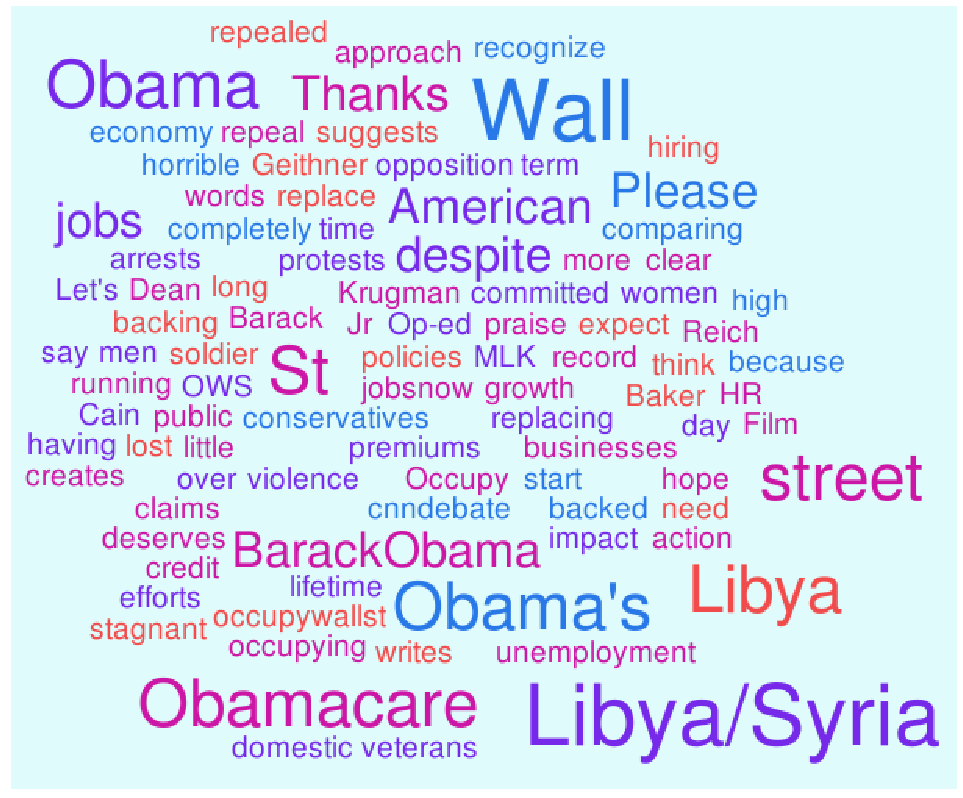
\includegraphics[width=2.4in,height=1.8in]{example.pdf}
\caption{Word Cloud of the User.}
\label{fig5}
\end{figure}
Figure~\ref{fig6} is the visualized subjectivity model of the user in a $ [0,100] $ topic space and a $ [0,8] $ sentiment valence space, which is constructed according to our method. 
\begin{figure}[htb]
\centering
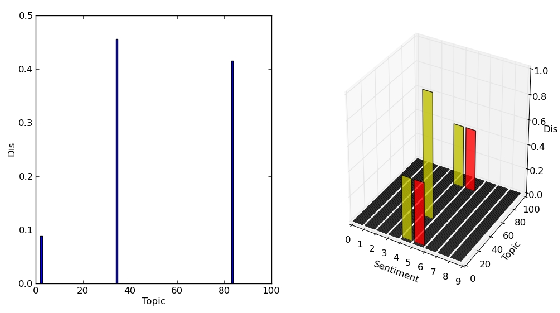
\includegraphics[width=3.8in,height=1.8in]{fig1.pdf}
\caption{Subjectivity model example. The left subgraph denotes interests distribution on topic 2, 32 and 83: $ (  w_{u}\left( 2 \right)=0.08,w_{u}\left( 32 \right)=0.48, w_{u}\left( 83 \right)=0.44)  $. The right subgraph denotes opinions towards topics: $ O_{2}=( d_{u,2} \left( 4 \right)=0.5, d_{u,2} \left( 5 \right)=0.5)$, $O_{32}=(d_{u,32} \left( 4 \right)=1.0) $, $ O_{83}=( d_{u,83} \left( 4 \right)=0.5, d_{u,83} \left( 5 \right)=0.5 ) $.}
\label{fig6}
\end{figure}
It is obvious that the user is interested in three topics (topic 2: ``\#Obamacare'', topic 32: ``\#libya'' and topic 83:``\#occupywallst''), and  the left part of Figure~\ref{fig6} denotes the weights of his topics of interest. The right part denotes the opinions towards three topics of the user, in which he is neutral to topic ``\#libya'' with 100\% distribution on sentiment strength value 4, positive to topic ``\#Obamacare'' and ``\#occupywallst'' with 50\% on value 4 and 50\% on value 5. 
From the example, it is demonstrated that our model can give a detail description for the subjectivity of users in that it can model not only the interest distribution but also opinion coverage over a fine-grain sentiment. To the best of our knowledge, generative models such as TSM and JST can only give relative coverage over positive, negative and neutral sentiment polarities.

\subsection{Link Prediction Performance}
It is hard for us to directly evaluate the effectiviness of our model quantitatively, therefore we adopt link prediction of social network analysis as an applicable task to test our model and comare our model with TSM and JST model. When a user forms a link in a network such as Twitter, then the principle of homophily \cite{lazarsfeld_friendship_1954}, or ``birds of a feather flock together'' \cite{mcpherson2001birds} —suggests that users that are``connected'' may tend to hold similar opinions \cite{thelwall2010emotion}. The connection a user creates may correspond to approval or a desire to pay attention, or suggestive of the possibility of a shared opinion. Therefore we calculate the content similarity between two users as a measurement to predict whether they will connect to each other. For the content similarity we calculate three kinds of similarities including the words similarity with bag-of-words model, the topic similarity with LDA model and subjectivity similarity with our model,TSM model and JST model. As for the subjectivity similarity, we mean both topic and opinion similarity between two users by adding them together. In our experiment, we adopt cosine similarity to calculating the similarities.

We randomly select 10,000 target users from our dataset with at least 80 followers. The followers of a target user is regard as positive instances, and the same number of non-followers are sampled as negative instances for that user. We combine all positive and negative instances into a balanced test dateset, and calculate three kinds of similarities between every target user and their test users as features for a supervised classifier. We adopt logistic classifier and run Leave-One-Out Cross-Validation (LOOCV) 100 times for each user to normalize the results. The finnal performance is evaluated by averaging all results of the 10,000 users. Accuracy is used as our performance measurement, and the result is list in Table~\ref{}
\begin{table}[htb]
\centering
\caption{Accuracy performance. BOW denotes words similarity, LDA denotes topic similarity, and SUB,TSM, JST denotes subjectivity similarity with our model, TSM and JST model separately. A significant improvement over BOW with $ \ast $ and LDA with $ \ddagger $ ($p < 0.05$).}
\label{tab3}
\begin{tabular}{|l|l|}
\hline
Feature & Accuracy(\%)\\
\hline
BOW & 55.85  \\
LDA & 61.76 $ \ast  $\\
TSM & 70.94  $ \ast \quad \ddagger $\\
JST & 66.25 $ \ast \quad \ddagger $\\
SUB & 71.53 $ \ast \quad \ddagger $\\
\hline
\end{tabular}
\end{table}
As can be observed from the result table that: firstly, the performance of bag-of-words model is the lowest with 55.85\% accuracy, and we think the reseason lying in the sparsity of tweets caused by informal usage of language by different users, if topic model is applied, the sparsity is lessened by clustering different words into one topic; secondly, if topic related opinions are considered, the prediction accuracy is improved significantly from only topic similarity in that all three models (TSM 70.94\%, JST 66.25\% and SUB 71.53\%) outperform the LDA model; finally, compared with two generative models, our model (SUB) outperforms JST significantly, and get a little better performance than TSM but the improvement is not significant, we think it is because sentiment analysis of our model is more suitable for the Twitter language, for it can extract subltle sentiment imbeded in special language characteristcs such as repeated letters and emoticons. Furthermore, our model can output more fine-grain opinions than just three porlarities, which can catch more fine opinion similarity between users.

\section{Conclusion}
\label{sec6}

In this paper, we study a novel opinion integration problem of social media usrs.
We propose a Subjectivity Model to solve this problem in a separated framework. Users’ historical messages are leveraged to construct their topic related opinions through topic model and sentimetn analysis techniques. With this model, we can automatically generate an integrated opinion summary that consists of both topic of interest distribution and topic related opinion distribution for a user. The proposed model is compared with generative models such as TSM and JST model to show that it is more suitable for the social media language. We experimented on Twitter data and the results show that the proposed Subjectivity model can effectively model topic related opinion with two probabilistic distributions and clearly outperforms generative models in a link prediction task.
In the future, we will apply our model in several social network analysis applications to testify its effectiveness.

\bibliographystyle{splncs}
\bibliography{apweref}
\end{document}
